% Szkielet dla pracy pisanej w języku angielskim.

\documentclass[polish,a4paper,twoside]{ppfcmthesis}

\usepackage[utf8]{inputenc}
\usepackage[OT4]{fontenc}
\usepackage{listings}
\usepackage{amsfonts}
\usepackage{amsmath}

\author{Szymon Dolata}                              % Your name comes here
\title{Integracja drzew prefiksowych w przetwarzaniu zbiorów zapytań eksploracyjnych algorytmem Apriori}        % Note how we protect the final title phrase from breaking
\ppsupervisor{Dr inż. Marek Wojciechowski} % Your supervisor comes here.
\ppyear{2014}                                         % Year of final submission (not graduation!)


\begin{document}

% Front matter starts here
\frontmatter\pagestyle{empty}%
\maketitle\cleardoublepage%

\pagebreak

% Blank info page for "karta dyplomowa"
\thispagestyle{empty}\vspace*{\fill}%
\begin{center}Tutaj przychodzi karta pracy dyplomowej;\\oryginał wstawiamy do wersji dla archiwum PP, w pozostałych kopiach wstawiamy ksero.\end{center}%
\vfill\cleardoublepage%

\pagebreak

% Table of contents.
\pagenumbering{Roman}\pagestyle{ppfcmthesis}%
\begingroup 
\renewcommand{\vspace}[2]{}% Gobble 2 arguments after \vspace
\tableofcontents* 
\endgroup
\cleardoublepage%

% Main content of your thesis starts here.
\mainmatter%
\chapter{Wstęp}
\label{c1}

\section{Integracja drzew prefiksowych w przetwarzaniu zbiorów zapytań eksploracyjnych algorytmem Apriori}
\label{c11}


Odkrywanie zbiorów częstych i generowanie na ich podstawie reguł asocjacyjnych, to problem sformułowany w kontekście analizy koszyka zakupów. Głównym celem jest szukanie prawidłowości w zachowaniu klientów supermarketów. Szybko znalazł on również zastosowanie w wielu innych dziedzinach, takich jak chociażby analiza działalności firm wysyłkowych, sklepów internetowych etc. Z wykorzystaniem znalezionych zbiorów częstych i wygenerowanych reguł dąży się do tego aby możn było wynioskować (z dużym prawdopodobieństwem), że niektóre produkty współwystępują ze sobą. Informacje takie, zwłaszcza jeśli wyrażone w formie zasad, często mogą być stosowane w celu zwiększenia sprzedanych danych produktów - na przykład poprzez odpowiednie rozmieszczenie ich na półkach w supermarkecie lub na stronach katalogu wysyłkowego (umieszczenie obok siebie może zachęcić jeszcze więcej klientów do zakupu ich razem) lub poprzez bezpośrednie sugerowanie klientom produktów, którymi mogą być zainteresowani. 

Oczywistym jest, że należy szukać tylko takich reguł asocjacyjnych, które są wiarygodne i niosą ze sobą jakąś informację. Istnieją wskaźniki służące do oceny tychże reguł. Zostały one omówione bardziej szczegółowo w rozdziale 2. 

Głównym problemem indukcji reguł asocjacyjnych jest to, że istnieje bardzo wiele możliwości. Przykładowo w zakresie produktów z supermarketu, których może być nawet kilka tysięcy, istnieją miliardy możliwych reguł. Tak ogromna ilość nie może być przetwarzana sekwencyjnie. Dlatego potrzebne są wydajne algorytmy, które ograniczają przestrzeń wyszukiwania i sprawdzają jedynie podzbiór wszystkich reguł. Jednym z takich algorytmów jest Apriori opracowany przez \cite{Agrawal}.

Podstawowy algorytm Apriori trzyma kandydatów w drzewie haszowym. W ostatnich latach zaproponowane zostały metody Common Counting (\cite{WojciechowskiCC}) oraz Common Candidate Tree (\cite{WojciechowskiCCT}). Są one wynikiem badań nad optymalizacją wykonania kilku zadań Apriori uruchomionych współbieżnie na nakładających się podzbiorach tabeli z danymi. Metody sprowadzały się do:\newline
- Integracji odczytów współdzielonych danych z dysku;\newline
- Integracji drzew haszowych w jedno drzewo gdzie kandydaci mają kilka liczników (po jednym dla zadania eksploracji).\newline
W praktyce jednak lepsze okazały się implementacje Apriori gdzie drzewo haszowe zastąpiono znacznie prostszą strukturą drzewa prefiksowego. Powstało kilka rozwiązań wykorzystujacych tę strukturę: Borgelt, Bodon, Goethals. Jednak do tej pory nie została zaimplementowana modyfikacja Common Counting i Common Candidate Tree dla Apriori z drzewem prefiksowym i to właśnie jest celem tej pracy. 

\section{Cel i zakres pracy}
\label{c12}

Tak jak wspomniano, ogolnym celem pracy jest implementacja dwóch algorytmów wykonania zbioru zapytań odkrywających zbiory częste - które dotychczas implementowne były na drzewie haszowym - z wykorzystaniem drzew prefiksowych. \newline
Na ten ogólny cel pracy składają się następujące cele szczegółowe:
- przedstawienie, analiza i porównanie istniejących rozwiązań dotyczących tematyki pracy
- implementacja modyfikacji Common Counting i Common Candidate Tree dla Apriori z drzewem prefiksowym;\newline
- przetesotowanie wydajności zaimplementowanych algorytmów.\newline

\section{Opis infrastruktury}
\label{c13}
Algorytmy napisane zostały w języku Java, z wykorzystaniem narzędzia Maven oraz środowiska programistycznego Eclipse. Dane testowe generowane były za pomocą generatora GEN (\cite{AgrawalGEN}), a następnie wczytywane do bazy PostgreSQL, z której korzystała aplikacja. Tetsy przeprowadzone zostały na komputerze HP Envy 14 Notebook PC, z procesorem Intel Core i5-2410M 2x2.30GHz oraz 8GB pamięci RAM, pracujacym pod kontrola systemu operacyjnego Microsoft Windows 7. 
	
\section{Struktura pracy}
\label{c14}   
Struktura pracy jest następująca:\newline
-- w rozdziale 2 omówiono podstawowe pojęcia i definicje wykorzystywane w pracy;\newline
-- w rozdziale 3 przedstawiono istniejące rozwiązania i algorytmy, związane z tematem pracy;\newline
-- w rozdziale 4 przedstawiono ideę, opis i cechy alogrytmu;\newline
-- w rozdziale 5 przeanalizowano działanie algorytmu dla różnych parametrów i danych wejściowych;\newline
-- w rozdziale 6 przedstawiono winoski i uwagi do pracy.
\chapter{Podstawowe pojęcia i definicje}
\label{c2}

\section{Wstęp}
\label{c21}

W poniższym rozdziale omówiono podstawowe pojęcia i definicje wykorzystywane w pracy. 

\section{Lista pojęć i definicji}
\label{c22}

\subsection{Transakcja i element transakcji}
\label{c221}
Danymi wejściowymi dla odkrywania zbiorów częstych i reguł asocjacyjnych jest zbiór transakcji zdefiniowanych na zbiorze elementów. Tymi elementami mogą być produkty w sklepie, usługi, książki etc. Ważne jest, aby te elementy można było w łatwy sposób od siebie odróżnić. Jeśli \( I = \{ i_1, i_2, \cdots, i_n \}\)  (ang. \textit {item base} ), to zbiór wszystkich możliwych elementów, to dowolny niepusty podzbiór X zbioru \(X\subseteq I\) nazywamy transakcją (ang. \textit{itemset}). Natomiast zbiór elementów o mocy \textit{k}, to taki zbiór, który posiada dokładnie k elementów (ang. \textit{k-itemset}). Mówi się, że 

Transakcja jest zatem przykładowym zbiorem elementów, np. zbiorem produktów, które zostały kupione przez danego klienta. Jako że transakcje mogą się powtarzać (może istnieć kilku klientów, którzy kupili dokładnie takie same produkty), to nie ma możliwości żeby zamodelować wszystkie możliwe transakcje (koszyki). Wynika to z tego, że elementy w zbiorze nie mogą się powtarzać. Problem ten znalazł kilka rozwiązań. Należy do nich zamodelowanie wszystkich transakcji jako multizbioru (uogólnienie pojęcia zbioru, w którym w odróżnieniu od klasycznych zbiorów jeden element może występować wiele razy) albo jako wektora (elementy na różnych pozycjach mogą być takie same, ale wyróżnia je położenie). Innym - choć podobnym do wspomnianego wyżej zastosowania wektora - rozwiązaniem jest rozszerzenie każdej transakcji o unikalny identyfikator. Kolejną możliwością jest wykorzystanie zbioru unikalnych transakcji, z tą różnicą, że do każdej transakcji przypisany jest licznik mający za zadanie zliczanie wystąpień.

Należy także zwrócić uwagę, że w większości rozważanych przypadków nie są znane wszystkie elementy, jakie mogą znaleźć się w zbiorze \(I\). Przyjmuje się wówczas, że ten zbiór jest sumą elementów występujacych we wszystkich transakcjach.

\subsection{Reguła asocjacyjna}
\label{c222}
Reguła asocjacyjna jest implikacją, która daje możliwość przewidywania jednoczesnego wystąpienia dwóch zjawisk i zachowań, współzależnych od siebie. Innymi słowy jest to schemat, pozwalający - z określonym prawdopodobieństwem - założyć, że jeśli nastąpiło zdarzenie A, to nastąpi również zdarzenie B. W kontekście problemu koszyka zakupów sprowadza się do reguł w stylu: \textit{Jeżeli klient kupił pieluszki, to (z określonym prawdopodobieństem) kupi też piwo.}

\subsection{Wsparcie transakcji}
\label{c223}
Jeśli \(T\) oznacza jedną z transakcji w zbiorze wszystkich transakcji \(D\), to (bezwzgędne) wsparcie tej transakcji jest równe \(U\) - liczbie wystąpień \(T\) w zbiorze \(D\). Wsparcie względne jest to z kolei procent (lub ułamek) transakcji w zbiorze \(D\), które zawierają \(T\). Obliczamy ze wzoru \[sup_{rel}(T)=\nolinebreak\frac{|U|}{|D|}*100\%\]. Dla algorytmu Apriori określa się próg minimalnego wsparcia \(minsup\), który również może być wyrażony w dwojakiej postaci - jako liczba wystąpień lub procent wszystkich transakcji. W poszukiwaniu zbiorów częstych interesujące są tylko te reguły, dla których \(sup(T) \geq minsup \), gdzie \(sup(T)\), to przyjęty w pracy sposób zapisu wsparcia transakcji \(T\) w rozważanym zbiorze transakcji \(D\).

\subsection{Ufność reguły asocjacyjnej}
\label{c224}
Ufność reguły asocjacyjnej jest miarą jakości danej reguły. Miara ta została przedstawiona przez autorów algorytmu Apriori \cite{Agrawal1994}. Dla reguły asocjacyjnej postaci \(R = "X\rightarrow Y"\) (gdzie \(X\) i \(Y\) to zbiory elementów) ufność wyraża się jako stosunek wspracia sumy wsystkich elementów występujących w regule (w tym przypadku \(sup(X \cup Y)\)) do wstparcia poprzednika reguły (tutaj \(sup(X)\)). 
\[conf(R) = \frac{sup(X \cup Y)}{sup(X)}\]
Należy dodać, że nie ma znaczenia czy wykorzystywane jest wsparcie aboslutne czy relatywne. Istotne jest natomiast to, aby w zarówno dla licznika i mianowika wykorzystany był ten sam typ wsparcia.
Z powyższego wzoru wynika, że ufność reguły asocjacyjnej, to stosunek liczby przypadków, w których jest ona poprawna, do wszystkich przypdków gdzie mogłaby zostać zastosowana.
Przykład: \(R = wino \wedge chleb \rightarrow ser\) - jeśli klient kupuje wino i chleb, to ta reguła ma zastowanie i mówi, że można oczekiwać, że dany klient kupi również ser. Jest możliwe, że ta reguła - dla danego klienta - będzie poprawna lub nie. Interesują informacją jest to jak dobra jest reguła, czyli jak często jest poprwana (jak często klient, króty kupuje wino i chleb kupuje również ser). Taką właśnie informację uzyskuje się poprzez obliczenie ufności reguły asocacyjnej. Oczywiście w przypadku gdy klient nie kupił chleba lub/i wina, to reguła nie znajduje zastowania, a dana transakcja nie wpływa na \(conf(R)\). 

\subsection{Wsparcie reguły asocjacyjnej}
\label{c225}
Wsparcie reguły asocjacyjnej postaci \(A \cup B \rightarrow C\) odpowiada wsparciu zbioru \(S = \{A, B, C\}\) (\cite{Agrawal}).Miara ta informuje o tym jak często dana reguła jest prawidłowa. Nieco odmienna definicja została przedstawiona i wykorzystana w \cite{Borgelt}. Różnica polega na tym, że wpsarcie wyrażone jest jako liczba przypdków, w których reguła jest stosowalna. Zatem dla powyżej postaci byłoby to \(S = \{A, B\}\), nawet jeśli reguła może okazać się fałszywa. 
Wparcie może być stosowane do filtrowania. Dla ustalonego \(minsup\) szuka się tylko takich reguł, których wsparcie jest nie mniejsze od \(minsup\). Oznacza to, że interesujące są tylko te reguły, które wystąpiły co najmniej daną liczbę razy.
W algorytmach wyszukiwania reguł asocjacyjnych stosuje się progi mnimalnego wsparcia oraz mnimalnej ufności. Dzięki temu w otrzymanych wynikach nie są uwzględnione mało wartościowe reguły.

\subsection{Zbiór częsty}
\label{c226}
Zbiorem częstym nazywamy taki niepusty podzbiór zbioru \(I\), dla którego wsparcie jest równe co najmniej wartości \(minsup\).

\subsection{Zbiór domknięty}
\label{c227}
Zbiorem domkniętym nazywamy taki zbiór częsty, dla którego nie istnieje żaden nadzbiór mający dokładnie takie samo wsparcie.

\subsection{Zbiór maksymalny}
\label{c228}
Zbiorem maksymalnym nazywamy taki zbiór częsty, dla którego nie istnieje żaden nadzbiór, który byłby zbiorem częstym.

\subsection{Zapytanie eksploracyjne}
\label{c229}

\subsection{Zbiór elementarnych predykatów selekcji danych dla zbioru zapytań eksploracyjnych}
\label{c2210}
\chapter{Podłoże teoretyczne}
\label{c3}

\section{Wstęp}
\label{c31}
Kolejny rozdział przedstawia aktualne metody i istniejące algorytmy związane z tematem pracy. Poza podstawowym algorytmem Apriori (\cite{Agrawal}), który używa drzew haszowych do przechwywania kandydatów, opisano trzy modyfikacje tego alogrytmu. Główna różnica polega na tym, że wykorzystują one inną strukturę, a mianowicie drzewa prefiksowe. Są to rozwiązania zaproponowane przez Christina Borgelta (\cite{Borgelt}), Ferenca Bodona (\cite{Bodon}) oraz Barta Goethalsa (\cite{Goethals}). Ze względu na wykorzystanie prostszej struktury okazały się one szybsze od standardowego algorytmu.
 
Innym problemem jest optymalizacja wykonania kilku zadań Apriori uruchomionych współbieżnie na nakładających się podzbiorach tabeli z danymi. Metody z tym związane to Common Counting (\cite{WojciechowskiCC}) i Common Candidate Tree (\cite{WojciechowskiCCT}). Oparte są one o implementację Apriori z zastosowaniem drzew haszowych. Brakuje jednak adaptacji tych algorytmów, polegającej na zmianie struktury na drzewa prefiksowe. Właśnie taka modyfikacja została wprowadzona, a uzyskane efekty opisano w kolejnych rozdziałach niniejszej pracy. 


\section{Przegląd istniejących rozwiązań}
\label{c32}

\subsection{Algorytm Apriori \cite{Agrawal}}
\label{c321}
Algorytm Apriori jest algorytmem eksploracji poziomej. Szuka zbiorów częstych o rozmiarach \(1, 2,\dots , k\). Algorytm rozpoczyna od zbiorów o rozmiarze 1 i następnie zwiększa ten rozmiar w kolejnych iteracjach. Elementy każdej transakcji są uporządkowane leksykograficznie - jeżeli nawet transakcje nie są posortowane, to krokiem wstępnym algorytmu może być leksykograficzne uporządkowanie elementów transakcji (\cite{Morzy}). Po pierwszym kroku zebrane są zatem wszystkie elementy występujące w transakcjach (w postaci zbiorów jednolementowych). Następnie sprawdzane jest, które z nich posiadają wsparcie nie mniejsze niż \(minsup\). Elementy niespełniające tego wymgania są odrzucane. Pozostałe służą do utworzenia dwuelementowych zbiorów kandydujących (ang. \textit{candidate itemsets}). Dla wygenerowanych zbiorów spradzane jest czy posiadają wsparcie równe co najmniej \(minsup\). Jeśli tak, to taki zbiór jest dodawany do listy zbiorów częstych i w kolejnej iteracji jest wykorzystywany (wraz z innymi zbiorami z tejże listy) do generowania zbiorów kandydatów o rozmiarze o 1 większym. Wsparcie zbiorów sprawdzane jest na podstawie odczytu danych z bazy danych. Algorytm zatrzymuje się gdy nie ma już możliwości generowania kolejnych zbiorów. W wyniku jego działania zwracana jest suma \(k\)-elementowych zbiorów częstych \((k = 1, 2,\dots)\), która może zostać wykozystana do generowania reguł asocjacyjnych.

\subsection{Algorytm Apriori - implementacja Christina Borgelta \cite{Borgelt}}
\label{c322}

\subsection{Algorytm Apriori - implementacja Ferenca Bodona \cite{Bodon}}
\label{c323}

\subsection{Algorytm Apriori - implementacja Barta Goethalsa \cite{Goethals}}
\label{c324}


\subsection{Common Counting \cite{WojciechowskiCC}}
\label{c325}
Integracja odczytów współdzielonych danych z dysku

\subsection{Common Candidate Tree \cite{WojciechowskiCCT}}
\label{c326}
Integracja drzew haszowych w jedno drzewo gdzie kandydaci mają kilka liczników (po jednym dla zadania eksploracji)
\chapter{Opracowane algorytmy}
\label{c4}

\section{Wstęp}
\label{c41}

Whatever

\section{Common Steps}
\label{c42}

Whatever
\chapter{Wyniki eksperymentów}
\label{c5}

\section{Wstęp}
\label{c51}
W poniższym rozdziale opisano przebieg przeprowadzonych eksperymentów oraz przedstawiono uzyskane wyniki wraz z ich interpretacją. Algorytmy testowane były na tych samych zbiorach danych. Tworzenie tych zbiorów odbywało się z wykorzystaniem generatora przyjmującego jako parametry liczbę transakcji (np. 10 tys., 100 tys.), średnią liczbę elementów w transakcji (np. 6), liczbę wzorców do odkrycia (np. 500), średni rozmiar wzorców częstych do odkrycia (np. 3), liczbę różnych elementów występujących w transakcjach (np. 1000, 10000) oraz nazwę pliku wyjściowego. Wygenerowany plik jest importowany do bazy danych, do której odwołuje się aplikacja podczas wykonywania algorytmów. Dane w bazie składowane są w jednej tabeli w postaci par \((id transakcji, id elementu)\). Dlatego też po odczycie tej tabeli składane są transakcje wykorzystywane w dalszym przetwarzaniu. Zbiór zapytań \(DMQ\) generowany był przed rozpoczęciem przetwarzania. Liczba transakcji obejmująca każde zapytanie \(dmq_i\) wynosi \(|T|/|DMQ|\), gdzie \(|T|\) - liczba wszystkich transakcji, \(|DMQ|\) - liczba wszystkich zapytań eksploracyjnych. 

\section{Opis infrastruktury}
\label{c52}
Algorytmy napisane zostały w języku Java, z wykorzystaniem narzędzia Maven oraz środowiska programistycznego Eclipse. Dane testowe generowane były za pomocą generatora GEN (\cite{AgrawalGEN}), a następnie wczytywane do bazy PostgreSQL, z której korzystała aplikacja. Testy przeprowadzone zostały na komputerze HP Envy 14 Notebook PC, z procesorem Intel Core i5-2410M 2x2.30GHz oraz 8GB pamięci RAM, pracującym pod kontrola systemu operacyjnego Microsoft Windows 7. 

\section{Wyniki}
\label{c53}
Poniżej zaprezentowano wyniki eksperymentów. Wszystkie uwzględnione czasy są średnią 4 dokonanych pomiarów dla dokładnie tych samych parametrów. Badania przeprowadzono dla dwóch zapytań eksploracyjnych z różnym poziomem nakładania się danych. Oba zapytania wykorzystywały ten sam próg wsparcia, mimo że nie jest to wymaganiem algorytmu. Jest to podyktowane chęcią możliwości lepszego zaobserwowania różnic w działaniu algorytmów niezależnie od wykorzystywanych progów dla poszczególnych zapytań. Algorytmy uwzględniane w wynikach to Common Counting z wykorzystaniem drzew prefiksowych (CCP), Common Candidate z wykorzystaniem drzew prefiksowych (CCTP) oraz sekwencyjnie wykonywana adaptacja algorytmu Apriori (SEQ) zgodna z tą zastosowaną wewnątrz CCP i CCTP.

Zbiór danych 1. Parametry generatora dla drugiego zbioru danych przedstawia tabela \ref{table:firstDataSetParams}.
\begin{table}[h]
\begin{center}
	\begin{tabular}{| l | c |}
		\hline
		liczba transakcji & 100000 \\ \hline
		średnia liczba elementów w transakcji & 8 \\ \hline
		liczba różnych elementów & 1000 \\ \hline
		liczba wzorców (zbiorów częstych) & 1500 \\ \hline
		średnia liczba elementów we wzorcu & 4 \\ 
		\hline
	\end{tabular}
\end{center}
\caption{Parametry generatora dla pierwszego testowego zbioru transakcji.}
\label{table:firstDataSetParams}
\end{table}

\begin{figure}[h]
	\centering
	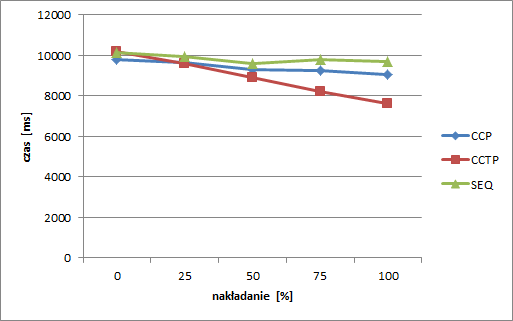
\includegraphics[width=0.8\linewidth]{figures/chart_100_2}
	\caption{Wykres dla pierwszego zbioru danych dla dwóch zapytań \(dmq\) z różnym stopniem nakładania się i \(minsup = 2\%\)}
	\label{fig:chart_100_2}
\end{figure}

Na wykresie \ref{fig:chart_100_2} zestawione czasy trwania poszczególnych algorytmów wykonywanych na pierwszym zbiorze danych z różnymi stopniami nakładania się. Przyjęta wartość \(minsup\) dla wszystkich zapytań wynosiła 2\%. Jak widać na wykresie w przypadku braku nakładania się zapytań uzyskane czasy były do siebie bardzo zbliżone. Wraz ze wzrostem stopnia nakładania się uwidaczniały się różnice w czasach wykonania algorytmów. Wykonanie sekwencyjne cały czas utrzymywało się na niemalże takim samym poziomie. Jest to związane z podobną liczbą operacji wykonywaną w trakcie działania algorytmu. W przypadku CCP i CCTP wraz ze wzrostem nakładania zwiększała się współbieżność. W przypadku CCTP skrócenie czasu następuje szybciej niż ma to miejsce dla CCP. Jednakże dla CCP także zaobserwowany został stały spadek czasu wykonania. Można powiedzieć, że dla tego przypadku algorytm CCTP okazał się zdecydowanie najlepszy, a także zastosowanie CCP zamiast SEQ skutkowało krótszym czasem udzielenie odpowiedzi na zadane zapytania eksploracyjne.

\begin{figure}[h]
	\centering
	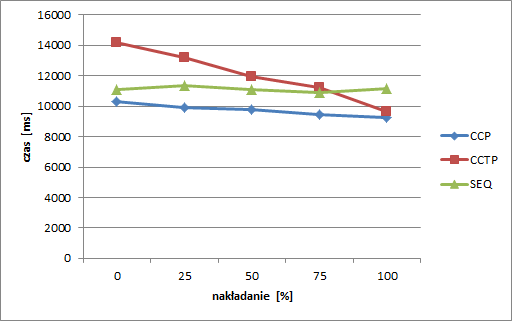
\includegraphics[width=0.8\linewidth]{figures/chart_100_1}
	\caption{Wykres dla pierwszego zbioru danych dla dwóch zapytań \(dmq\) z różnym stopniem nakładania się i \(minsup = 1\%\)}
	\label{fig:chart_100_1}
\end{figure}
Drugi rozważany przypadek na pierwszym zbiorze danych został przedstawiony na wykresie~\ref{fig:chart_100_1}. Przyjęto \(minsup\) ma poziomie 1\%. Mniejsza wartość progu minimalnego wsparcia przekłada się na większą liczbę zbiorów częstych odkrywanych w trakcie wykonań algorytmów, stąd też wydłużenie czasów wykonania. W przypadku wykonania sekwencyjnego po raz kolejny widoczny jest brak wpływu nakładania się zapytań eksploracyjnych. Podobnie jak w pierwszym analizowanym przykładzie zachowuje się algorytm Common Counting. Widoczne jest skracanie czasu wykonania wraz ze wzrostem nakładania się zapytań. Jest to zależność liniowa i mimo, że przyspieszenie nie jest bardzo znaczące, to po raz kolejny CCP działa szybciej niż SEQ. Ciekawa sytuacja została zaobserwowana dla Common Candidate Tree. Znowu widoczny jest stały, liniowy spadek czasu wykonania, ale tym razem algorytm dla większości rozważanych przypadków nakładania się \(dmq\) działa wolniej. Jest to zapewne spowodowane koniecznością sprawdzania kolejności (i sortowania jeśli jest to niezbędne) elementów w danym wierzchołku (problem ten opisany został w \ref{c46}). Nie było to widoczne dla \(minsup = 2\%\) ze względu na mniejszą liczbę zbiorów częstych na każdym poziomie drzewa, co ma bezpośrednie przełożenie na liczbę kandydatów na kolejnym poziomie, a więc liczbę dodawanych do drzewa wierzchołków. Mimo to dla znaczącego nakładania się obserwowany jest zysk względem SEQ. 


Zbiór danych 2. Parametry generatora dla drugiego zbioru danych przedstawia tabela \ref{table:secondDataSetParams}. 
\begin{table}[h]
	\begin{center}
		\begin{tabular}{| l | c |}
			\hline
			liczba transakcji & 50000 \\ \hline
			średnia liczba elementów w transakcji & 8 \\ \hline
			liczba różnych elementów & 1000 \\ \hline
			liczba wzorców (zbiorów częstych) & 1000 \\ \hline
			średnia liczba elementów we wzorcu & 4 \\ 
			\hline
		\end{tabular}
	\end{center}
	\caption{Parametry generatora dla drugiego testowego zbioru transakcji.}
	\label{table:secondDataSetParams}
\end{table}

\begin{figure}[h]
	\centering
	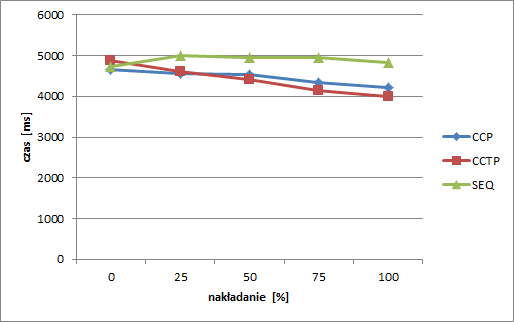
\includegraphics[width=0.8\linewidth]{figures/chart_50_2}
	\caption{Wykres dla drugiego zbioru danych dla dwóch zapytań \(dmq\) z różnym stopnieniem nakładania się i \(minsup = 2\%\)}
	\label{fig:chart_50_2}
\end{figure}
Wykres \ref{fig:chart_50_2} obrazuje czasy wykonania algorytmów dla mniejszego z wygenerowanych zbiorów danych, na których przeprowadzane były testy. Podobnie jak miało to miejsce w uprzednio opisanych przypadkach czasy wykonania SEQ są niemalże liniowe. Zaobserwowane drobne różnice wynikają prawdopodobnie z tego, że zapytania odnoszą się do różnych podzbiorów zbioru danych, a także wpływem chwilowych różnic w działaniu środowiska testowego. Patrząc na wyniki uzyskane przez CCP o CCTP okazuje się, że są one bardzo zbliżone. Po raz kolejny czas wykonania maleje szybciej dla Common Candidate Tree niż dla Common Counting. Jednakże dla przyjętych dla tej obserwacji parametrów ciężko jednoznacznie wskazać algorytm lepszy, aczkolwiek oba są szybsze od algorytmu sekwencyjnego. 

\begin{figure}[h]
	\centering
	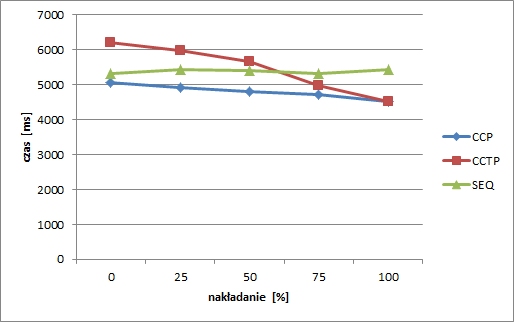
\includegraphics[width=0.8\linewidth]{figures/chart_50_1}
	\caption{Wykres dla drugiego zbioru danych dla dwóch zapytań \(dmq\) z różnym stopnieniem nakładania się i \(minsup = 1\%\)}
	\label{fig:chart_50_1}
\end{figure}
Na wykresie \ref{fig:chart_50_1} zaprezentowano wyniki uzyskane dla drugiego zbioru danych przy założeniu, że próg minimalnego wsparcia wynosi \(1\%\). Potwierdza on niezależność wykonania sekwencyjnego względem stopnia nakładania się zapytań \(dmq_i\). Obserwowane rezultaty dla CCP i CCTP przypominają te uzyskane dla pierwszego zbioru danych i \(minsup = 1\%\). Widoczny jest dłuższy czas wykonania CCTP, w stosunku do SEQ i CCP, dla zapytań nie nakładających się lub małego stopnia nakładania. Powodem jest tak jak poprzednio konieczność wykonywania większej liczby sprawdzeń kolejności elementów w wierzchołku (i ewentualnych sortowań). Nie zmienia to faktu, że widoczny jest stały spadek czasu wykonania wraz ze wzrostem współbieżności. Z kolei Common Counting potwierdza swoją przewagę nad wykonaniem sekwencyjnym oraz fakt, że zwiększanie stopnia nakładania się zapytań działa na rzecz skrócenia (proporcjonalnie do zwiększania się nakładania) przetwarzania \(DMQ\) tym algorytmem. 

\section{Porównanie CCP i CCTP z CC i CCT}
\label{c54}
Powołując się na wyniki uzyskane w \cite{WojciechowskiCC} oraz \cite{WojciechowskiCCT} można stwierdzić, że zastosowanie Common Counting wykorzystującego struktury prefiksowe daje podobny efekt jak w przypadku drzew haszowych. Efektem tym jest stały wzrost szybkości przetwarzania proporcjonalny do stopnia nakładania się danych. Nieco inaczej rzecz ma się dla Common Candidate Tree. Po zmianie drzewa haszowego na prefiksowe dla algorytmu nadal obserwowany jest liniowy (szybszy niż dla CC) spadek czasu wykonania. Niestety w przypadkach gdy na każdym poziomie drzewa generowanych jest dużo kandydatów (np. stosunkowo małe \(minsup\)) i nie występuje duże nakładanie się zapytań, to algorytm ten traci swoją przewagę. Jest to przewaga CCT (\cite{WojciechowskiCCT}), gdyż dla drzewa haszowego kolejność dodawania wierzchołków nie ma wpływu na przetwarzanie.


\chapter{Wnioski i uwagi}

Przeprowadzone eksperymenty pokazują, że nie da się łatwo zaadoptować algorytmów przetwarzania zbiorów zapytań eksploracyjnych (Common Counting \cite{WojciechowskiCC} i Common Candidate Tree \cite{WojciechowskiCCT}) opartych na oryginalnym Apriori (\cite{Agrawal}) do rozwiązań korzystających z zoptymalizowanych wersji algorytmu Apriori wykorzystujących drzewa prefiksowe. Mimo to jest to 

Badany obszar pozostawia bardzo dużo możliwości i perspektyw do prowadzenia dalszych prac nad optymalizacją wykonania zarówno zbioru zapytań eksploracyjnych, jak i samego algorytmu Apriori. 

% All appendices and extra material, if you have any.
\cleardoublepage\appendix%
\chapter{Zawartość płyty DVD}

Jako dodatek do tego dokumentu dołączona jest płyta DVD. Zawiera ona materiały związane z prezentowanym tematem w formacie elektronicznym dla osób, które mogą być zainteresowane kontynuacją prac w tym temacie. 

Płyta DVD zawiera następujące elementy:

\begin{enumerate}
\item Elektroniczna wersja pracy magisterskiej w formacie PDF jak i w formacie do edycji (TEX).
\item Aplikacja konsolowa w języku Java z zaimplementowanymi algorytmami.
\item Generator danych testowych.
\end{enumerate}


% Bibliography (books, articles) starts here.
\bibliographystyle{alpha}{\raggedright\sloppy\small\bibliography{bibliography}}

% Colophon is a place where you should let others know about copyrights etc.
\ppcolophon

\end{document}
